\chapter{ชื่อของบท....}

\section{หัวข้อแรก..........}
เนื้อหาแรก....... \Gls{Example}

\subsection{หัวข้อย่อยที่ 1 .....ของหัวข้อแรก}
เนื้อหาย่อยของหัวข้อแรก latex\index{latex} \textcite{haverbeke2018eloquent}

\subsection{หัวข้อย่อยที่ 2 .....ของหัวข้อแรก}
เนื้อหาย่อยของหัวข้อแรก


\section{หัวข้อที่ 2 ..........}
เนื้อหาแรก.......

\subsection{หัวข้อย่อยที่ 1 .....ของหัวข้อที่ 2}
เนื้อหาย่อยของหัวข้อแรก

\subsection{หัวข้อย่อยที่ 2 .....ของหัวข้อที่ 2}
เนื้อหาย่อยของหัวข้อแรก


\begin{figure}
    \centering
    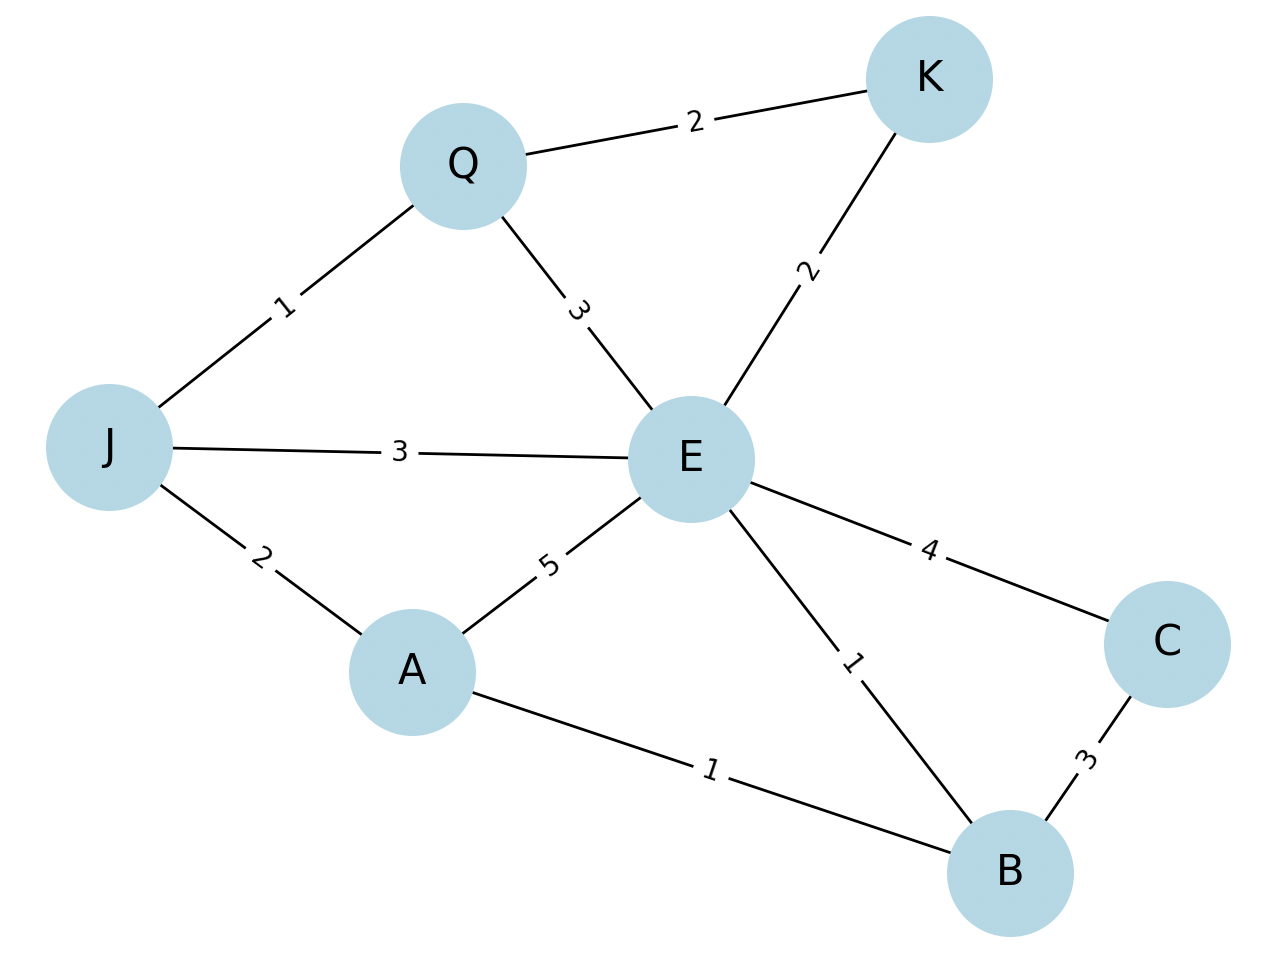
\includegraphics[width=0.5\linewidth]{author//images/graph.png}
    \caption{ใส่ชื่อภาพ}
    \label{fig:enter-label}
\end{figure}
